\section{Problemformulering}
\label{sec:problemformulering}

PTS opbygges til tracking og nedskydning af en lerdue i English Skeet (ES). PTS dimensioneres til en konkurrence i ES og er afgrænset til et enkelt tilfælde:
Afskydning fra ”high house” med PTS placeret på station 4 (B), jf. figur \ref{fig:ES}.
\begin{figure}[th!]
\centering
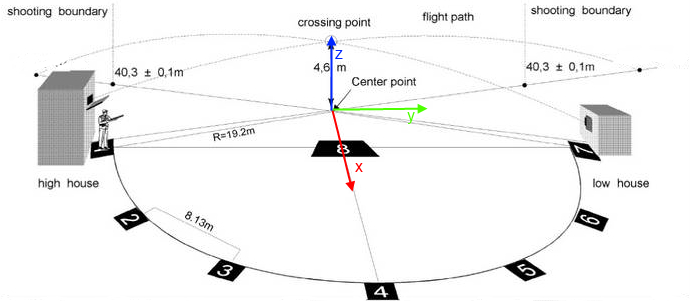
\includegraphics[width=1\textwidth]{./graphics/skeet_diagram_cropped_axes}
\caption[Skitse af ES]{Optegning af skyttepositioner samt lerduens flugt fra de to affyringsstationer hhv. "high house", "Low House". PTS er placeret på position 4.}
\label{fig:ES}
\end{figure}	

Udgangsposition for PTS er at systemet peger mod "high house" (D) hvorfra lerduen afskydes.
%GL:
%Trackingen skal forestille at have til formål at assistere i nedskydningen af lerduen,
%og man skal således forestille sig et gevær monteret på tilt-rammen:
%Et tænkt masseløst gevær placeret i skæringspunktet mellem pan- og tilt-akserne står vinkelret
%på tilt-planet, og skal skyde lerduen jf. reglerne for ES, dvs. inden lerduen når "shooting boundary", figur \ref{fig:ES}.
%Da man har to skud til rådighed, er det et krav at trackingen foretaget af PTS har stabiliseret sig på lerduen
%i tide, så man kan nå at affyre to skud. 

Til nedskydning af lerduen er et tænkt masseløst gevær placeret i skæringspunktet mellem pan- og tilt-akserne.
Geværet er monteret vinkelret på tilt-planet. 
Lerduen skal skydes iht. reglerne for ES, dvs. inden lerduen når "shooting boundary" (SB), figur \ref{fig:ES}.
%\todo[inline, author=Michael]{En figur der viser geværet på PTS ville være meget velkommen}
%\todo[inline, author=Michael]{Jeg har udkommenteret sætningen om 2 skud, da vi jævnfør paragraf 4.21 i regelsættet kun må affyre et skud per lerdue. Desuden er resten afsnittet omskrevet. (Det står dog gemt i kommentarerne)}

Det tænkte gevær er et 12 gauge haglgevær med Skeet Choke.

Lerduens koordinater i det kartesiske koordinatsystem som vist på figur \ref{fig:ES}
vil med en frekvens på 120 [Hz] blive givet som input til systemet. 
Hvor disse koordinater stammer fra er uden for projektafgrænsningen.

Som angivet i projektoplægget skal reguleringen foregå på en mikrocontroller,
mens motorpositionsbestemmelse skal foregå på en FPGA.